\justify
\fontsize{12pt}{14}\
\setlength{\parindent}{0cm}

\section{Actividad 3}
\normalsize El producto seleccionado para realizar los gráficos de oferta y demanda fue la yuca, esto se debe a que es uno de los productos más consumidos y producidos del departamento de Sucre la región en donde vivo. Así lo deja claro lo mencionado por \cite{hochschild2024} que menciona que solo en el munucipio de Corozal la yuca corresponde a tres cuartas partes de la producción total de estos tipos de cultivo. Así pues, tal cómo se evidencia en la figura \ref{fig:demanda} de la página \pageref{fig:demanda}, la demanda de este tubérculo varía de acuerdo al precio, de este modo a medida que el precio disminuye la demanda aumenta y viceversa. De igual modo, en la figura \ref{fig:oferta} de la página \pageref{fig:oferta} se observa que a medida que los precios aumentan la oferta aumenta y viceversa.

\begin{figure}[ht!]
    \centering
    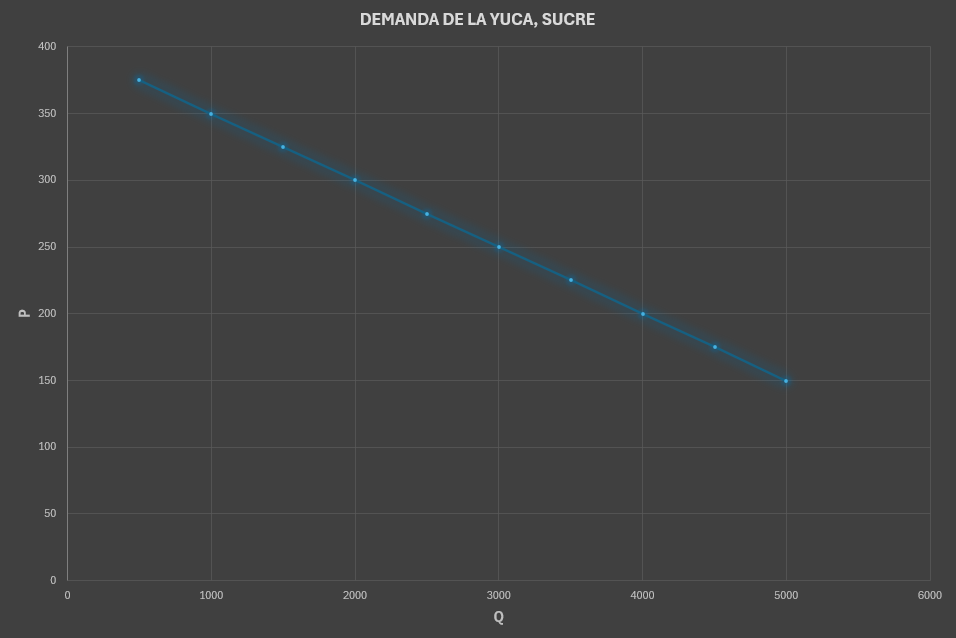
\includegraphics[width=15cm, height=13cm]{Demanda de la yuca}
    \caption{Diagrama de la demanda de la yuca en Sucre}
    \label{fig:demanda}
\end{figure}

\begin{figure}[ht!]
    \centering
    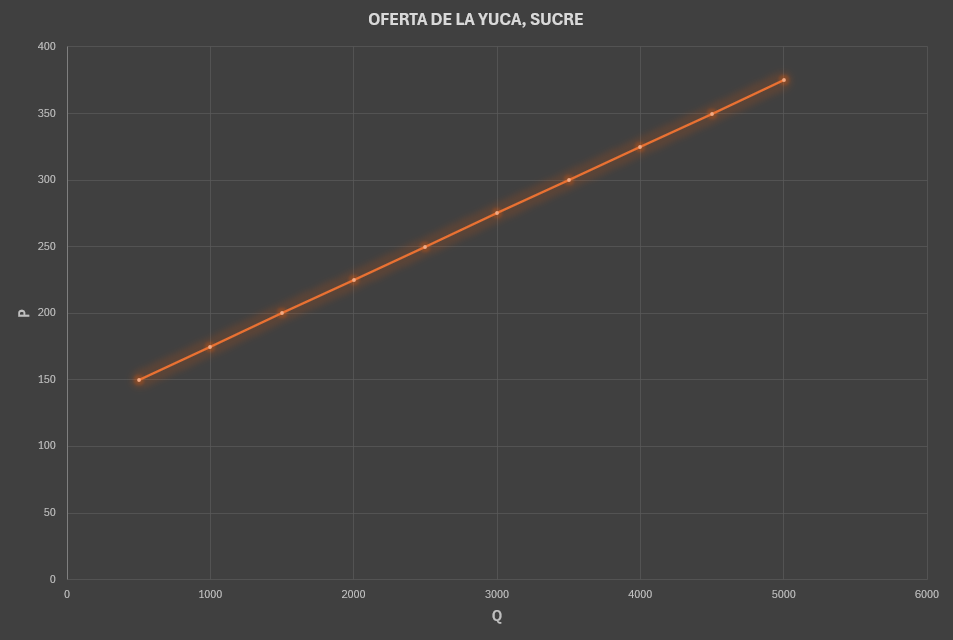
\includegraphics[width=15cm, height=13cm]{Oferta de la yuca}
    \caption{Diagrama de la oferta de la yuca en Sucre}
    \label{fig:oferta}
\end{figure}